\documentclass{standalone}
\usepackage{graphicx}	
\usepackage{amssymb, amsmath}
\usepackage{color}

\usepackage{tikz}
\usetikzlibrary{intersections, backgrounds, math}
\usepackage{pgfmath}

\definecolor{light}{RGB}{220, 188, 188}
\definecolor{mid}{RGB}{185, 124, 124}
\definecolor{dark}{RGB}{143, 39, 39}
\definecolor{highlight}{RGB}{180, 31, 180}
\definecolor{gray10}{gray}{0.1}
\definecolor{gray20}{gray}{0.2}
\definecolor{gray30}{gray}{0.3}
\definecolor{gray40}{gray}{0.4}
\definecolor{gray60}{gray}{0.6}
\definecolor{gray70}{gray}{0.7}
\definecolor{gray80}{gray}{0.8}
\definecolor{gray90}{gray}{0.9}
\definecolor{gray95}{gray}{0.95}


\begin{document}

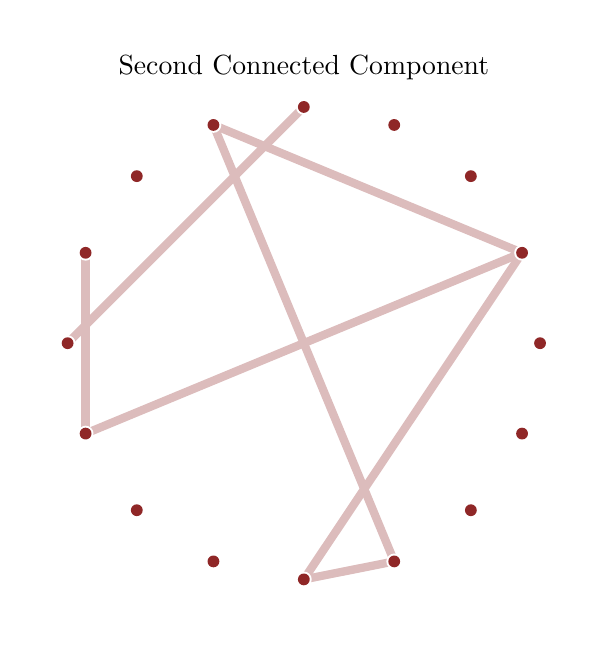
\begin{tikzpicture}[scale=1]
  \pgfmathsetmacro{\R}{3};
    
  \begin{scope}[shift={(14, 0)}]
    \draw[white] (-3.5, -3.5) rectangle (3.5, 4);
    
    % Component Two
    % 1, 4, 5, 7, 8, 9, 12, 13
    \foreach \ni/\nf in {1/5, 1/9, 1/12, 4/8, 5/13, 7/9, 12/13} {
      \pgfmathsetmacro{\thetai}{360 * (\ni / 16)};
      \pgfmathsetmacro{\thetaf}{360 * (\nf / 16)};
      
      \draw[light, line width=3]    
           ({ \R * cos(\thetai) }, { \R * sin(\thetai)} )
        -- ({ \R * cos(\thetaf) }, { \R * sin(\thetaf)} );
    }
    
    \foreach \n in {0, 1, ..., 15} {
      \pgfmathsetmacro{\theta}{360 * (\n / 16)};
      
      \fill[white] ({ \R * cos(\theta) }, { \R * sin(\theta)} ) circle (0.1);
      \fill[dark]  ({ \R * cos(\theta) }, { \R * sin(\theta)} ) circle (0.075);
    }
    
    \node at (0, 3.5) { Second Connected Component };
  \end{scope}
  
\end{tikzpicture}

\end{document}  